\documentclass[12pt,openany]{book}


\usepackage{amsmath,amsthm,amsfonts,amscd} % Packages for mathematics
\usepackage{url}
\usepackage{booktabs}

% Colors
\usepackage[dvipsnames]{xcolor}
\definecolor{titleblue}{RGB}{0,53,128}
\definecolor{chaptergray}{RGB}{140,140,140}
\definecolor{sectiongray}{RGB}{180,180,180}

\definecolor{thmcolor}{RGB}{231, 76, 60}
\definecolor{defcolor}{RGB}{52, 152, 219}
\definecolor{lemcolor}{RGB}{155, 89, 182}
\definecolor{corcolor}{RGB}{46, 204, 113}
\definecolor{procolor}{RGB}{241, 196, 15}

% Fonts
\usepackage[T1]{fontenc}
\usepackage[utf8]{inputenc}
\usepackage{newpxtext,newpxmath}
\usepackage{sectsty}
\allsectionsfont{\sffamily\color{titleblue}\mdseries}

% Page layout
\usepackage{geometry}
\geometry{a4paper,left=1.5in,right=1in,top=1in,bottom=1in,heightrounded}
\usepackage{fancyhdr}
\fancyhf{}
\fancyhead[LE,RO]{\thepage}
\fancyhead[LO]{\nouppercase{\rightmark}}
\fancyhead[RE]{\nouppercase{\leftmark}}
\renewcommand{\headrulewidth}{0.5pt}
\renewcommand{\footrulewidth}{0pt}

% Chapter formatting
\usepackage{titlesec}
\titleformat{\chapter}[display]
{\normalfont\sffamily\Huge\bfseries\color{titleblue}}{\chaptertitlename\ \thechapter}{20pt}{\Huge}
\titleformat{\section}
{\normalfont\sffamily\Large\bfseries\color{titleblue!100!gray}}{\thesection}{1em}{}
\titleformat{\subsection}
{\normalfont\sffamily\large\bfseries\color{titleblue!50!gray}}{\thesubsection}{1em}{}

% Table of contents formatting
\usepackage{tocloft}
\renewcommand{\cftchapfont}{\sffamily\color{titleblue}\bfseries}
\renewcommand{\cftsecfont}{\sffamily\color{chaptergray}}
\renewcommand{\cftsubsecfont}{\sffamily\color{sectiongray}}
\renewcommand{\cftchapleader}{\cftdotfill{\cftdotsep}}

% Hyperlinks
\usepackage{hyperref}
\hypersetup{
	colorlinks=true,
	linkcolor=titleblue,
	filecolor=black,      
	urlcolor=titleblue,
}

%---------------------------My Preamble
\usepackage{graphicx}
\usepackage{tikz-cd}
\usepackage{pgfplots}
\usetikzlibrary{positioning}
\usetikzlibrary{calc}
\usetikzlibrary{decorations.markings}
\usepackage{enumerate}

\usepackage{xcolor}
\usepackage{cancel}
\newcommand\crossout[3][black]{\renewcommand\CancelColor{\color{#1}}\cancelto{#2}{#3}}
\newcommand\ncrossout[2][black]{\renewcommand\CancelColor{\color{#1}}\cancel{#2}}
\usepackage{soul}
\newcommand{\mathcolorbox}[2]{\colorbox{#1}{$\displaystyle #2$}}


%Tcolorbox
\usepackage[most]{tcolorbox}
\newcommand{\mycolorbox}[3]{%
	\begin{center}
		\begin{tcolorbox}[colback=white,colframe=#1,arc=10pt,title={\color{white}\textbf{#2}}]
			#3%
		\end{tcolorbox}
	\end{center}
}
\tcbset{colback=white, arc=5pt}
%\tcbset{colback=white,colframe=black,fonttitle=\bfseries,arc=4mm,boxrule=1pt,shadow={2mm}{-1mm}{0mm}{black!50}}
%\tcbset{enhanced, colback=white,colframe=blue!50!black,fonttitle=\bfseries,arc=4mm,boxrule=1pt,shadow={2mm}{-1mm}{0mm}{black!50}}
%drop shadow

%White box with black text and shadow
%\begin{tcolorbox}[colback=white,colframe=black,fonttitle=\bfseries,title=Black Shadow Box,arc=4mm,boxrule=1pt,shadow={2mm}{-1mm}{0mm}{black!50}]
%	This is a white box with black text and a subtle shadow. The shadow adds some depth and dimension to the box without overpowering the design.
%\end{tcolorbox}

%Theorem
%\usepackage{amsthm}
\newtheorem{axiom}{Axiom}[section]
\newtheorem{theorem}{Theorem}[chapter]
\newtheorem{proposition}[theorem]{Proposition}
\newtheorem{corollary}{Corollary}[theorem]
\newtheorem{lemma}[theorem]{Lemma}

\theoremstyle{definition}
\newtheorem{definition}{Definition}[chapter]
\newtheorem{remark}{Remark}[section]
\newtheorem{note}{Note}[section]
\newtheorem{exercise}{Exercise}[section]
\newtheorem{example}{Example}[section]

%New Command
\newcommand{\set}[1]{\left\{#1\right\}}
\newcommand{\N}{\mathbb{N}}
\newcommand{\Z}{\mathbb{Z}}
\newcommand{\Q}{\mathbb{Q}}
\newcommand{\R}{\mathbb{R}}
\newcommand{\C}{\mathbb{C}}
\newcommand{\F}{\mathbb{F}}
\newcommand{\nbhd}{\mathcal{N}}

\newcommand{\of}[1]{\left( #1 \right)} 
\newcommand{\abs}[1]{\left\lvert #1 \right\rvert}
\newcommand{\norm}[1]{\left\| #1 \right\|}
\newcommand{\inv}[1]{{#1}^{-1}}

\newcommand{\sol}{\textcolor{magenta}{\bf Sol}}
\newcommand{\conjugate}[1]{\overline{#1}}

\renewcommand{\Re}{\operatorname{Re}}
\renewcommand{\Im}{\operatorname{Im}}

\newcommand{\ie}{\textnormal{i.e.}}

% Begin document
\begin{document}
	
	% Title page
	\begin{titlepage}
		\begin{center}
			{\Huge\textsf{\textbf{Complex Analysis}}\par}
			\vspace{0.5in}
			{\Large Ji Yong-Hyeon\par}
			\vspace{1in}
			%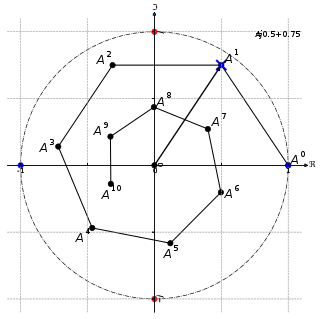
\includegraphics[width=3in]{Exponentials_of_complex_number_within_unit_circle-2.png}
			\begin{tikzpicture}[scale=1.8,>=Stealth]
				% draw axes
				\draw[->, thick, black] (-2,0) -- (2,0) node[below right, black] {$\Re$};
				\draw[->, thick, black] (0,-2) -- (0,2) node[above left, black] {$\Im$};
				
				% draw unit circle
				\draw[blue, thick] (0,0) circle (1.4cm);
				
				% draw point
				\filldraw[red] (1,1) circle (0.08cm) node[anchor=south west, black] {$z = a + ib$};
				
				% draw radius
				\draw[dashed, thick, red] (0,0) -- (1,1) node[midway, above left, black] {$r$};
				
				% draw angle
				\draw[->, thick, orange] (0.3,0) arc (0:45:0.3) node[midway, right, black] {$\theta$};
			\end{tikzpicture}\par
			\vspace{1in}
			{\large Ji Yong-Hyeon\par}
			{\large \today\par}
		\end{center}
	\end{titlepage}
	
	% Table of contents
	\tableofcontents
	
	% Chapters
	\mainmatter
	
	\chapter*{Continuity and Derivatives}
	
	\section*{Continuity}
	\begin{tcolorbox}[title=Continuity]
		\begin{definition}
			Let $\varnothing\neq S(\subseteq\R)$. Let $f:S\to\R$ be a real function, and let $\alpha\in S$. We say that \textbf{$f$ is continuous at $\alpha$} if \[
			\forall\varepsilon>0:\exists\delta>0\quad\text{s.t.}\quad\abs{x-\alpha}<\delta\implies\abs{f(x)-f(\alpha)}<\varepsilon.\footnote{$\iff \forall\varepsilon>0:\exists\delta>0\ \text{s.t.}\ f\left(\nbhd_\delta(\alpha)\right)\subseteq\nbhd_\varepsilon\left(f(\alpha)\right)$.}
			\] In other words, \[
			\lim\limits_{x\to\alpha}f(x)=f(\alpha).
			\] If $f$ is continuous on every point of $S$, then $f$ is called a \textbf{continuous function on $S$}.
		\end{definition}
	\end{tcolorbox}
	\begin{remark}
		$f$ is discontinuous at $\alpha$ if and only if \begin{align*}
			&\exists\varepsilon>0\quad\text{s.t.}\quad\forall\delta>0:\abs{x-\alpha}<\delta\ \text{but}\ \abs{f(x)-f(\alpha)}\geq\varepsilon\\
			\iff &\exists\varepsilon>0\quad\text{s.t.}\quad\forall\delta>0:\nbhd_\varepsilon\left(f(\alpha)\right)\subset f\left(\nbhd_\delta(\alpha)\right).
		\end{align*}
	\end{remark}
	
	
	\begin{tcolorbox}[colback=white!10!white,colframe=blue!50!black,title=Continuity]
		A function $f:S(\neq\varnothing)\to\R$ is continuous at $\alpha\in S$ iff \[
		\varepsilon\in\R^+\implies\exists\delta\in\R^+:[f\left[\nbhd_\delta\of{\alpha}\right]\subseteq\nbhd_\varepsilon\of{f\of{\alpha}}].
		\]
	\end{tcolorbox}
	
	\begin{tcolorbox}[colback=red!5!white,colframe=red!75!black,title=Warning]
		This is a warning box. It can be used to alert readers to potential dangers or problems.
	\end{tcolorbox}
	
	\begin{tcolorbox}[colback=white!10!white,colframe=black!50!white,title=Tabular Box,fonttitle=\bfseries\large,sharp corners]
		\begin{tabular}{|c|c|c|}
			\hline
			1 & 2 & 3 \\
			\hline
			4 & 5 & 6 \\
			\hline
			7 & 8 & 9 \\
			\hline
		\end{tabular}
	\end{tcolorbox}
	
	
	The continuity of a function is a fundamental concept that describes the behavior of a function near its domain. A function is said to be continuous at a point $x_0$ in its domain if the limit of the function as $x$ approaches $x_0$ exists and is equal to the function value at $x_0$.
	
	The formal definition of continuity of a function $f(x)$ at a point $x_0$ is:
	
	\begin{align*}
		\lim_{x \to x_0}f(x) &= f(x_0)\
	\end{align*}
	
	That is, the limit of $f(x)$ as $x$ approaches $x_0$ exists and is equal to $f(x_0)$.
	
	If a function is continuous at every point in its domain, then it is said to be a continuous function. There are different types of continuity, such as pointwise continuity, uniform continuity, and local continuity.
	
	Pointwise continuity means that the function is continuous at each point in its domain. Uniform continuity means that the function has a continuous behavior over the entire domain, without any abrupt changes or jumps. Local continuity means that the function is continuous in a small neighborhood around each point in its domain.
	
	The concept of continuity is important in the analysis of functions, and it plays a crucial role in the study of limits, derivatives, and integrals. The continuity of a function also helps us understand its behavior, including the existence of critical points, extreme values, and asymptotic behavior.
	
	In summary, the continuity of a function is a crucial concept in mathematical analysis, and it is essential for understanding the behavior of functions near their domain.
	
	\newpage
	\section{Derivatives}
	\begin{tcolorbox}[title=Differentaible Mapping]
		\begin{definition}
			Let $f:I\to\R$ on an interval $I$ and $\alpha\in I$. A real function $f$ \textbf{is differentiable at the point $\alpha$} if and only if either the limit \[
			f'(\alpha):=\frac{df}{dx}\bigg|_{x=\alpha}:=\mathcolorbox{-blue}{\lim_{x\to\alpha}\frac{f(x)-f(\alpha)}{x-\alpha}}\quad\text{or}\quad \mathcolorbox{-blue}{\lim_{h\to0}\frac{f(\alpha+h)-f(h)}{h}}
			\] exists. Here, $x=\alpha+h$. The real number $f'(\alpha)\in\R$ is the \textbf{derivative of $f$ at the point $\alpha$}.
		\end{definition}
	\end{tcolorbox} 
	\begin{remark}
		A real number $f'(\alpha)\in\R$ is the derivative of $f$ at $\alpha$ if \[
		\varepsilon>0\implies\exists\delta>0: f\left({\nbhd_\delta}^*(\alpha)\right)\subseteq \nbhd_\varepsilon\left(f'(\alpha)\right).
		\]
	\end{remark}
	\
	\begin{tcolorbox}[colback=white]
		\begin{theorem}
			Let $f:I\to\R$ be a real function defined on an interval $I$, and let $\alpha\in I$. \[
			\text{$f$ is differentiable at $\alpha$}\implies\text{$f$ is continuous at $\alpha$}.
			\] In other words, \[
			\exists\lim_{x\to\alpha}\frac{f(\alpha)-f(x)}{x-\alpha}\implies\lim_{x\to\alpha}f(x)=f(\alpha).
			\]
		\end{theorem}
	\end{tcolorbox}
	\begin{proof}
		By hypothesis, $f'(\alpha)$ exists. We have, then, \begin{align*}
			\lim_{x\to\alpha}\left(f(x)-f(\alpha)\right)&=\lim_{x\to\alpha}\left[\frac{f(x)-f(\alpha)}{(x-\alpha)}(x-\alpha)\right]\\
			&=\lim_{x\to\alpha}\frac{f(x)-f(\alpha)}{(x-\alpha)}\cdot\lim_{x\to\alpha}(x-\alpha)\\
			&=f'(\alpha)\cdot0\\
			&=0.
		\end{align*} Hence $\lim\limits_{x\to\alpha}f(x)=f(\alpha)$.
	\end{proof}
	
	
	\chapter{The Complex Number System}
	
	The complex number system is an extension of the real number system that includes a new type of number called the complex number. A complex number is a number that can be expressed in the form $a + bi$, where $a$ and $b$ are real numbers and $i$ is the imaginary unit, which is defined as the square root of $-1$.
	
	The real part of a complex number a + bi is a, and the imaginary part is b. We can represent complex numbers geometrically using the complex plane, which is a two-dimensional plane where the horizontal axis represents the real part of a complex number and the vertical axis represents the imaginary part.
	
	Addition and subtraction of complex numbers are performed by adding or subtracting their real and imaginary parts separately. Multiplication of complex numbers is performed using the distributive property and the fact that $i^2 = -1$. Division of complex numbers is also possible by multiplying both the numerator and denominator by the complex conjugate of the denominator.
	
	The absolute value or modulus of a complex number is the distance between the origin and the point representing the complex number on the complex plane. It is defined as:
	
	\begin{align*}
		|a+bi| &= \sqrt{a^2 + b^2}
	\end{align*}
	
	The argument or phase of a complex number is the angle that the line connecting the origin to the point representing the complex number makes with the positive real axis. It is defined as:
	
	\begin{align*}
		\theta &= \operatorname{arg}(a+bi) = \operatorname{arctan}\left(\frac{b}{a}\right)
	\end{align*}
	
	The complex number system is important in mathematics, physics, engineering, and many other fields. It is used to represent quantities that have both a magnitude and a direction, such as electrical currents and electromagnetic waves. Complex numbers also have applications in signal processing, control theory, and cryptography, among others.
	
	\newpage
	\section{The Field of Complex Numbers}
	
	The set of complex numbers, denoted by $\C$, is defined as the collection of all ordered pairs $(x,y)$ where $x,y\in\R$. The operations of addition and multiplication are defined by:\begin{align*}
		(x_1,y_1)+(x_2+y_2)&=(x_1+x_2,y_1+y_2),\\
		(x_1,y_1)\cdot(x_2+y_2)&=(x_1x_2-y_1y_2,x_1y_2+x_2y_1).\\
	\end{align*}
	
	We verify that the axioms for a field are met by the definitions given for $\C$: \begin{itemize}
		\item[(F1)] $\of{\C,+}$ is an "Abelian group",
		\item[(F2)] $\of{\C\setminus\set{0},\cdot}$ is an Abelian group, and
		\item[(F3)] the distributive law holds: $x,y,z\in\C\implies\of{x+y}\cdot z=x\cdot z+y\cdot z$.
	\end{itemize}
	
	In (F1), an Abelian group refers to the fact that the operation $+$ on $\C$ satisfies the properties of associativity and commutativity, and \[
	\exists e:=(0,0)\in\C:[(x,y)\in\C\implies(x,y)+e=(x,y)=e+(x,y)].
	\] Additionally, \[
	(x,y)\in\C\implies\exists(-x,-y)\in\C:[(x,y)+(-x,-y)=(0,0)=(-x,-y)+(x,y)].
	\] In condition (F2), the multiplicative identity is (1,0), and the multiplicative inverse of any complex number (x,y) in $\C\setminus\set{(0,0)}$ is determined by \begin{align}
		\of{\frac{x}{x^2+y^2},\frac{-y}{x^2+y^2}}.
	\end{align}
	
	\begin{exercise}
		Verify that (1.1) is indeed the inverse of $(x,y)\in\C\setminus\set{(0,0)}$.
		\begin{proof}[\sol]
			Let $(x,y)\in\C$. Then \begin{align*}
				(x,y)\cdot\of{\frac{x}{x^2+y^2},\frac{-y}{x^2+y^2}}
				&=\of{\frac{x^2}{x^2+y^2}-\frac{-y^2}{x^2+y^2},\frac{-xy}{x^2+y^2}+\frac{xy}{x^2+y^2}}\\
				&=\of{\frac{x^2+y^2}{x^2+y^2},\frac{-xy+xy}{x^2+y^2}}\\
				&=(1,0).
			\end{align*}
		\end{proof}
	\end{exercise}
	
	\begin{tcolorbox}[title=Complex Numbers are Field]
		\begin{proposition}
			$\of{\C,+,\cdot}$ is a field.
		\end{proposition}
	\end{tcolorbox}
	
	\newpage
	\section{Geometric Representation of Complex Numbers}
	\begin{center}
		\begin{tikzpicture}[scale=0.8]
			% draw axes
			\draw[->] (-4,0) -- (4,0) node[right] {$\Re(z)$};
			\draw[->] (0,-4) -- (0,4) node[above] {$\Im(z)$};
			% draw point
			\filldraw[black] (1.5,2) circle (2pt) node[anchor=south west] {$(x,y)$};
			% add arrow
			\draw[->] (0,0) -- (1.5,2) node[midway,above left] {};
			
		\end{tikzpicture}
	\end{center}
	
	\begin{center}
		\begin{tikzpicture}[scale=2]
			% axes
			\draw[->] (-1.5,0) -- (1.5,0) node[right] {$\text{Re}$};
			\draw[->] (0,-1.5) -- (0,1.5) node[above] {$\text{Im}$};
			
			% z1
			\draw[->,thick] (0,0) -- (1,1) node[above right] {$z_1$};
			\draw[dotted] (1,1) -- (1,0) node[midway,right] {$\operatorname{Im}(z_1)$};
			\draw[dotted] (1,1) -- (0,1) node[midway,above] {$\operatorname{Re}(z_1)$};
			\draw (0.3,0) arc (0:45:0.3) node[midway,right] {$\theta_1$};
			
			% z2
			\draw[->,thick] (0,0) -- (0.5,-1) node[below right] {$z_2$};
			\draw[dotted] (0.5,-1) -- (0.5,0) node[midway,right] {$\operatorname{Im}(z_2)$};
			\draw[dotted] (0.5,-1) -- (0,-1) node[midway,below] {$\operatorname{Re}(z_2)$};
			\draw (-0.3,0) arc (180:225:0.3) node[midway,left] {$\theta_2$};
			
			% z1*z2
			\draw[->,thick] (0,0) -- (0.5,1.5) node[above] {$z_1 \cdot z_2$};
			\draw[dotted] (0.5,1.5) -- (0.5,0) node[midway,right] {$\operatorname{Im}(z_1\cdot z_2)$};
			\draw[dotted] (0.5,1.5) -- (0,1.5) node[midway,above] {$\operatorname{Re}(z_1\cdot z_2)$};
			\draw (0.6,0) arc (0:67:0.6) node[midway,right] {$\theta_1+\theta_2$};
			
			% braces
			%\draw[decorate,decoration={brace,amplitude=5pt},xshift=-4pt,yshift=0pt]
			%(0.5,0) -- (0.5,1.5) node [black,midway,xshift=-8pt] {$r_1 r_2$};
			%\draw[decorate,decoration={brace,amplitude=5pt},xshift=0pt,yshift=4pt]
			%(0,1.5) -- (0.5,1.5) node [black,midway,yshift=10pt] {$r_1 r_2$};
		\end{tikzpicture}
	\end{center}
	
	\subsection{De Movire's formula and $n$th roots}
	\begin{tcolorbox}[title=De Moivre's Formula]
		\begin{proposition}
			Let $n\in\N$. Then \[
			\of{\cos\theta+i\sin\theta}^n=\cos(n\theta)+\sin(n\theta).
			\]  That is, \[
			n\in\N\implies \mathcolorbox{-blue}{\of{e^{i\theta}}^n=e^{in\theta}}.
			\]
		\end{proposition}
	\end{tcolorbox}
	
	\begin{exercise}
		By considering $(2+i)(3+i)$, show that \[
		\frac{\pi}{4}=\arctan\frac{1}{2}+\arctan\frac{1}{3}.
		\]
	\end{exercise}
	
	\begin{exercise}
		Let $a,z\in\C$ satisfy $\abs{a}<1$ and $\abs{z}\leq 1$. Prove that \[
		\abs{\frac{z-a}{1-\bar{a}z}}\leq 1.
		\] \begin{proof}[\sol]
			Note that $\abs{\frac{z-a}{1-\bar{a}z}} = \frac{\abs{z-a}}{\abs{1-\bar{a}z}}$. We have:
			\begin{align*}
				\abs{1-\bar{a}z}^2 &= (1-\bar{a}z)(1-\bar{a}z) \\
				&= 1 - \bar{a}z - a\bar{z} + \abs{a}^2 \abs{z}^2 \\
				&= (1-\abs{a}^2) - (\bar{a}z + a\bar{z}) + \abs{a}^2 \abs{z}^2 \\
				&= (1-\abs{a}^2) - 2\Re(\bar{a}z) + \abs{a}^2 \abs{z}^2 \\
				&= (1-\abs{a}^2)(1-\abs{z}^2),
			\end{align*} where we used the fact that $\abs{a}^2 = a\bar{a}$ and $\Re(\bar{a}z) = \frac{1}{2}(\bar{a}z + a\bar{z})$. Thus, we have:
			$$\abs{\frac{z-a}{1-\bar{a}z}} = \frac{\abs{z-a}}{\abs{1-\bar{a}z}} = \frac{\abs{z-a}}{\sqrt{1-\abs{a}^2}\sqrt{1-\abs{z}^2}} \leq 1$$
			since \begin{align*}
				\abs{a}<1\leadsto 1-\abs{a}^2> 0 \\
				\abs{z}\leq 1\leadsto 1-\abs{z}^2\geq 0
			\end{align*}$\abs{a}<1$ and $\abs{z}\leq 1$ imply that $1-\abs{a}^2\geq 0$ and $1-\abs{z}^2\geq 0$, and therefore, $\sqrt{1-\abs{a}^2}\geq 0$ and $\sqrt{1-\abs{z}^2}\geq 0$.
			
			Thus, we have shown that $\abs{\frac{z-a}{1-\bar{a}z}}\leq 1$.
		\end{proof}
	\end{exercise}
	
	\section{Convergence and continuity}
	
	\begin{tcolorbox}[colback=white,colframe=defcolor,arc=5pt,title={\color{white}\bf Limit of Complex function}]
		\begin{definition}
			Let $f: \Omega \subseteq \mathbb{C} \rightarrow \mathbb{C}$ be a complex function and $z_0 \in \mathbb{C}$ be a limit point of $\Omega$. We say that the limit of $f(z)$ as $z$ approaches $z_0$ is $L \in \mathbb{C}$ and write
			\[ \lim_{z \to z_0} f(z) = L \]
			if for every $\epsilon > 0$, there exists a $\delta > 0$ such that for all $z \in \Omega$ with $0 < |z - z_0| < \delta$, we have $|f(z) - L| < \epsilon$.
		\end{definition}
	\end{tcolorbox}
	
	\begin{tcolorbox}[colback=white,colframe=defcolor,arc=5pt,title={\color{white}\bf Continuity of Complex function}]
		\begin{definition}
			Let $f: \Omega \subseteq \mathbb{C} \rightarrow \mathbb{C}$ be a complex function and $z_0 \in \Omega$. We say that $f(z)$ is continuous at $z_0$ if for every $\epsilon > 0$, there exists a $\delta > 0$ such that for all $z \in \Omega$ with $|z - z_0| < \delta$, we have $|f(z) - f(z_0)| < \epsilon$.
			
			Equivalently, $f(z)$ is continuous at $z_0$ if and only if $\lim_{z \to z_0} f(z) = f(z_0)$.
			
			We say that $f(z)$ is continuous on $\Omega$ if $f(z)$ is continuous at every point in $\Omega$.
		\end{definition}
	\end{tcolorbox}
	
	\newpage
	\section{Domains}
	\begin{tcolorbox}[title=Path; Curve; Contour;]
		\begin{definition}
			A \textbf{path} (or \textbf{curve}) in $\C$ is a continuous function $\gamma:[a,b]\to\C$.
		\end{definition}
	\end{tcolorbox}
	
	\begin{tcolorbox}[title=Stepwise Path;]
		\begin{definition}
			A \textbf{path} (or \textbf{curve}) in $\C$ is a continuous function $\gamma:[a,b]\to\C$.
		\end{definition}
	\end{tcolorbox}
	
	\begin{tcolorbox}[title=Path-connected;]
		\begin{definition}
			An open set $U\subset\C$ is called \textbf{path-connected} if \begin{align*}
				\forall z_1,z_2\in U:\exists\text{a stepwise path}\ \gamma:[a,b]\to\C\ \text{s.t.}\ \gamma(a)=z_1,\gamma(b)=z_2\ \text{and}\\
				t\in[a,b]\implies\gamma(t)\in U.
			\end{align*}
		\end{definition}
	\end{tcolorbox}
	
	\newpage
	\section{The exponential function and its related objects}
	
	\subsection{The exponential $\exp z$}
	\begin{tcolorbox}[colback=white,colframe=defcolor,arc=5pt,title={\color{white}\bf Complex Exponential}]
		\begin{definition}
			The \textbf{complex exponential function} is defined as
			\begin{equation*}
				\exp{z} =\exp{(x+iy)} \triangleq e^{x}(\cos y + i\sin y),
			\end{equation*}
			where $x,y\in\R$ and $i$ is the imaginary unit, $i^2=-1$.
		\end{definition}
	\end{tcolorbox}
	\begin{remark}
		Recall that Taylor series $e^x=\sum_{n=0}^\infty\frac{1}{n!}x^n$. Note that \begin{align*}
			e^{iy}&=1+iy+\frac{1}{2!}(iy)^2+\frac{1}{3!}(iy)^3+\frac{1}{4!}(iy)^4+\frac{1}{5!}(iy)^5+\cdots\\
			&=\of{1-\frac{1}{2!}y^2+\frac{1}{4!}y^4-\cdots}+i\of{y-\frac{1}{3!}y^3+\frac{1}{5!}y^5-\cdots}\\
			&=\cos y+i\sin y.
		\end{align*} Then $e^{iy}=\cos y+i\sin y$. Thus, we have $
		\exp z=e^x(\cos y+i\sin y)=e^{x+iy}.
		$
	\end{remark}
	
	\begin{tcolorbox}[colback=white,colframe=procolor,arc=5pt,title={\color{white}\bf Properties of Complex Expoenential}]
		\begin{proposition}
			Let $z,z_1,z_2\in\C$. \begin{enumerate}[(1)]
				\item $\exp 0 = 1$.
				\item $\exp\of{z_1+z_2}=(\exp z_1)(\exp z_2)$.
				\item $\exp z\neq 0\implies\inv{\of{\exp z}}=\exp(-z)$.
				\item $\exp(z+2\pi i)=\exp z$.
				\item $\abs{\exp z}=e^{\Re\of{z}}$
			\end{enumerate}
		\end{proposition}
	\end{tcolorbox}
	\begin{proof}
		\begin{itemize}
			\item[(2)] Let $z_1=x_1+iy_1$ and $z_2=x_2+iy_2$. Then \begin{align*}
				\exp\of{z_1+z_2}=\exp\of{x_1+x_2+i(y_1+y_2)}&=e^{x_1+x_2+i(y_1+y_2)}\\
				&=e^{x_1+iy_1}e^{x_2+iy_2}\\
				&=\of{\exp z_1}\of{\exp z_2}.
			\end{align*}
			\item[(3)] $1=\exp 0=\of{\exp z}\of{\exp (-z)}$.
			\item[(4)] $\exp (z+2\pi)=e^z\of{\cos 2\pi+i\sin 2\pi}=\exp z(1+i\cdot 0)=\exp z$.
			\item[(5)] $\abs{\exp\of{z}}=\abs{e^x\cos y+e^x\sin y}=\sqrt{e^{2x}\cos^2y+e^{2x}\sin^2y}=e^x=e^{\Re\of{z}}$.
		\end{itemize}
	\end{proof}
	
	\newpage
	\subsection{Trigonometric functions}
	The complex exponential function is intimately connected to trigonometry. The trigonometric functions are defined using the complex exponential function. Let $x\in\R$ then \[
	\exp\of{ix}=\cos x+i\sin x\quad\text{and}\quad\exp\of{-ix}=\cos x-i\sin x.
	\] This gives
	\begin{equation*}
		\sin(x) = \frac{e^{ix} - e^{-ix}}{2i}
	\end{equation*} and
	
	\begin{equation*}
		\cos(x) = \frac{e^{ix} + e^{-ix}}{2}.
	\end{equation*}
	
	\newpage
	\subsection{Logarithm function}
	
	\begin{tcolorbox}[colback=white,colframe=defcolor,arc=5pt,title={\color{white}\bf Principal Agrugment}]
		\begin{definition}
			The \textbf{principal argument} of a complex number $z$, denoted by $\operatorname{Arg}(z)$, is defined to be the unique value $\theta \in (-\pi, \pi]$ such that $$
			z=\abs{z}e^{i\theta}=\abs{z}\of{\cos\theta+i\sin\theta}.
			$$
		\end{definition}
	\end{tcolorbox}
	
	The principal logarithm satisfies the following properties:
	
	\begin{itemize}
		\item $\operatorname{Log}(z_1 z_2) = \operatorname{Log}(z_1) + \operatorname{Log}(z_2)$ for all $z_1, z_2 \in \mathbb{C} \setminus (-\infty,0]$.
		\item $\operatorname{Log}(e^z) = z$ for all $z \in \mathbb{C}$.
		\item $\exp(\operatorname{Log}(z)) = z$ for all $z \in \mathbb{C} \setminus (-\infty,0]$.
	\end{itemize}
	\begin{tikzpicture}[scale=2]
		% Draw axes
		\draw[->] (-1.5,0) -- (1.5,0) node[right] {$\Re(z)$};
		\draw[->] (0,-1.5) -- (0,1.5) node[above] {$\Im(z)$};
		% Define clipping region
		\clip (0,0) circle (1);
		% Draw annulus
		\fill[gray!50] (0,0) circle ({1/sqrt(2)}) arc ({45}:{60}:{1/sqrt(2)}) -- (0,0);
		\fill[white] (0,0) circle ({1/sqrt(2)}) arc ({45}:{60}:{1/sqrt(2)});
		% Label annulus
		\node at ({1/sqrt(2)*cos(15)},{1/sqrt(2)*sin(15)}) {$\frac{\pi}{4}$};
		\node at ({1/sqrt(2)*cos(52.5)},{1/sqrt(2)*sin(52.5)}) {$\frac{\pi}{3}$};
	\end{tikzpicture}
	However, it's important to note that the principal logarithm is not continuous on the entire complex plane, since there is a branch cut along the negative real axis.
	
	The logarithm function is an important function in complex analysis that is defined as follows:
	
	Let $z$ be a non-zero complex number. Then the logarithm of $z$, denoted by $\log z$, is defined to be any complex number $w$ such that $e^w = z$.
	
	However, since $e^{w+2\pi i} = e^w$, there are infinitely many possible values of $\log z$. In fact, the set of all possible values of $\log z$ is given by
	\[ \log z = \ln|z| + i\arg z + 2\pi ik \]
	where $\ln|z|$ is the natural logarithm of the modulus of $z$, $\arg z$ is the argument of $z$, and $k$ is any integer.
	
	Note that the complex logarithm is not continuous on the entire complex plane, since there is a branch cut along the negative real axis. However, it is analytic on any simply connected domain that does not contain the origin.
	
	
	
	The principal logarithm of a complex number $z$, denoted by $\operatorname{Log}(z)$, is defined to be the complex number $w = \ln |z| + i \operatorname{Arg}(z)$.
	
	Note that the principal logarithm is a single-valued function defined on the domain $\mathbb{C} \setminus (-\infty,0]$.
	
	
	
	
	
	\newpage
	\begin{tikzpicture}[  node distance=1.5cm,  block/.style={    draw,    rectangle,    minimum width=2cm,    minimum height=1.5cm,    align=center  },  arrow/.style={    ->,    shorten >=2pt,    shorten <=2pt,  }]
		% Nodes
		\node[block] (G) {$G$};
		\node[block, below=of G] (H) {$H$};
		\node[block, below=of H] (K) {$K$};
		\node[block, right=of G] (GH) {$G \times H$};
		\node[block, right=of GH] (GK) {$G \times K$};
		\node[block, below=of GH] (HK) {$H \times K$};
		\node[block, below=of HK] (GHK) {$G \times H \times K$};
		% Arrows
		\draw[arrow] (G) -- (GH) node[midway,above] {$\varphi_G$};
		\draw[arrow] (H) -- (GH) node[midway,left] {$\varphi_H$};
		\draw[arrow] (K) -- (GK) node[midway,left] {$\varphi_K$};
		\draw[arrow] (GH) -- (GK) node[midway,above] {$\varphi_{GK}$};
		\draw[arrow] (GH) -- (HK) node[midway,left] {$\varphi_{HK}$};
		\draw[arrow] (HK) -- (GHK) node[midway,above] {$\varphi_{GHK}$};
		% Labels
		\node[left=of G] {$G$};
		\node[left=of H] {$H$};
		\node[left=of K] {$K$};
		\node[right=of GK] {$G \times K / \varphi_{HK}(H \times K)$};
		\node[below=of GH] {$G \times H / \varphi_{GK}(G \times K)$};
		\node[below=of HK] {$H \times K / \varphi_{GH}(G \times H)$};
		\node[below=of GHK] {$G \times H \times K / (\varphi_G(G) \times \varphi_H(H) \times \varphi_K(K))$};
	\end{tikzpicture}
	
	\begin{tikzpicture}[  node distance=2cm,  block/.style={    draw,    rectangle,    minimum width=3cm,    minimum height=1.5cm,    align=center  },  arrow/.style={    ->,    shorten >=2pt,    shorten <=2pt,  }]
		% Nodes
		\node[block] (Z) {$\mathbb{Z}$};
		\node[block, below=of Z] (Zn) {$\mathbb{Z}/n\mathbb{Z}$};
		\node[block, below=of Zn] (Zp) {$\mathbb{Z}/p\mathbb{Z}$};
		\node[block, right=of Z] (Zm) {$\mathbb{Z}/m\mathbb{Z}$};
		\node[block, right=of Zm] (Zmp) {$\mathbb{Z}/mp\mathbb{Z}$};
		% Arrows
		\draw[arrow] (Z) -- (Zn) node[midway,right] {$\pi_n$};
		\draw[arrow] (Zn) -- (Zp) node[midway,right] {$\pi_p$};
		\draw[arrow] (Z) -- (Zm) node[midway,above] {$\pi_m$};
		\draw[arrow] (Zm) -- (Zmp) node[midway,above] {$\pi_{mp}$};
		\draw[arrow] (Zn) -- (Zmp) node[midway,below] {$\phi_{n,p}$};
		% Labels
		\node[left=of Z] {$\mathbb{Z}$};
		\node[left=of Zn] {$\mathbb{Z}/n\mathbb{Z}$};
		\node[left=of Zp] {$\mathbb{Z}/p\mathbb{Z}$};
		\node[right=of Zmp] {$\mathbb{Z}/mp\mathbb{Z}$};
		\node[below=of Zn] {$\mathbb{Z}/np\mathbb{Z}$};
	\end{tikzpicture}
	
	\newpage
	\chapter{Complex Differentiability}
	
	\section{Complex Differentiability}
	\begin{tcolorbox}[colback=white,colframe=defcolor,arc=5pt,title={\color{white}\bf Complex Differentiability}]
		\begin{definition}
			A complex function $f:U(\subseteq\C)\to\C$, $U$ is an open subset, is said to be \textbf{complex differentiable} at a point $z_0\in U$ if $\exists f'(z_0)$ defined by\[
			f'(z_0)=\frac{df}{dz}\bigg|_{z=z_0}:=\mathcolorbox{-blue}{\lim_{z\to z_0}\frac{f(z)-f(z_0)}{z-z_0}}
			\]
		\end{definition}
	\end{tcolorbox}
	\begin{remark}
		We say that a complex function $f(z)$ is differentiable at a point $z_0\in U$ if \[
		\exists f'\of{z_0}\in\C:\left[\forall\varepsilon>0:\exists\delta>0:\forall z\in U:0<\abs{z-z_0}<\delta\Rightarrow\abs{\frac{f(z)-f(0)}{z-z_0}-f'(z_0)}<\varepsilon\right].
		\] 
	\end{remark}
	
	\begin{tcolorbox}[colback=white,colframe=lemcolor,arc=5pt,title={\color{white}\bf Equivalence of Complex Differentiability}]
		\begin{lemma}
			Let $U$ be an open set in $\C$, $z_0\in U$, and  $f:U\to C$. Then  the following are equivalent: \begin{enumerate}[(1)]
				\item $f$ is complex differentiable at $z_0$
				\item There exists an $r>0$, and function $h:D(z_0,r)\to\C$, where $D(z_0,r):=\set{z\in C:\abs{z-z_0}<r}$, such that \begin{itemize}
					\item[(a)] $f\of{z}=f\of{z_0}+[f'(z_0)+h(z)](z-z_0)$ for $\abs{z-z_0}<r$ and 
					\item[(b)] $\lim\limits_{z\to z_0}h\of{z}=0$.
				\end{itemize}
			\end{enumerate}
		\end{lemma}
	\end{tcolorbox}
	\begin{proof}
		\begin{itemize}
			\item[($\Rightarrow$)] Suppose that the complex derivative $f'(z_0)$ exists: \[
			f'(z_0) = \lim_{z \to z_0} \frac{f(z) - f(z_0)}{z - z_0}.
			\] We want to show that there an $r>0$ and a function $h:D\of{z_0,r}$ satisfying condition (a) and (b). Let $\varepsilon>0$. Define the function $h: D(z_0, \delta) \to \mathbb{C}$ by
			\[
			h(z) = \begin{cases}
				\frac{f(z) - f(z_0)}{z - z_0} - f'(z_0) &:z\neq z_0,\\
				0 &:z=z_0.
			\end{cases}
			\] Then \begin{itemize}
				\item[] (Case I) ($z\neq z_0$, \ie, $0<\abs{z-z_0}<\delta$) \begin{align*}
					h(z)=\frac{f(z) - f(z_0)}{z - z_0} - f'(z_0)\overset{\text{Rearraning}}{\implies}f\of{z}=f\of{z_0}+[f'(z_0)+h(z)](z-z_0).
				\end{align*}
				\item[] (Case II) ($z= z_0$, \ie, $0=\abs{z-z_0}$)\[
				f\of{z}=f\of{z_0}+[f'(z_0)+h(z)](z-z_0)\leftrightsquigarrow f\of{z_0}=f\of{z_0}+\crossout[red]{0}{[f'(z_0)+0]\cdot 0}.
				\]
			\end{itemize} Thus, $f\of{z}=f\of{z_0}+[f'(z_0)+h(z)](z-z_0)$ holds whenever $\abs{z-z_0}<\delta$. By the definition of $f'(z_0)$, we have
			\[
			\abs{\frac{f(z)-f(0)}{z-z_0}-f'(z_0)}=\abs{h}=\abs{h(z)-0}<\varepsilon.
			\]
			\item[($\Leftarrow$)] For $z\in D\of{z_0,r}\setminus\set{z_0}$, we have, upon rearranging, that \[
			\frac{f(z)-f(0)}{z-z_0}-f'(z_0)=h(z)\xrightarrow{z\to z_0} 0
			\] and so $\exists f'(z_0)$.
		\end{itemize}
		
		(<-) Conversely, suppose there exists an $r > 0$ and a function $h: D(z_0, r) \to \mathbb{C}$ satisfying conditions (a) and (b). We need to show that $f$ is complex differentiable at $z_0$.
		
		From condition (a), we have
		
		$f(z) = f(z_0) + [f'(z_0) + h(z)](z - z_0)$.
		
		Rearranging the terms and dividing by $(z - z_0)$, we obtain
		
		$\frac{f(z) - f(z_0)}{z - z_0} = f'(z_0) + h(z)$.
		
		Taking the limit as $z \to z_0$, we get
		
		$\lim_{z \to z_0} \frac{f(z) - f(z_0)}{z - z_0} = f'(z_0) + \lim_{z \to z_0} h(z)$.
		
		By condition (b), $\lim_{z \to z_0} h(z) = 0$. Thus,
		
		$f'(z_0) = \lim_{z \to z_0} \frac{f(z) - f(z_0)}{z - z_0}$.
		
		Since this limit exists, $f$ is complex differentiable at $z_0$.
		
		In conclusion, the function $f$ is complex differentiable at $z_0$ if and only if there exists an $r > 0$ and a function $h: D(z_0, r) \to \mathbb{C}$ satisfying conditions (a) and (b).
	\end{proof}
	
	
	\begin{tcolorbox}[colframe=procolor, title={\color{white}\bf }]
		\begin{proposition}
			Let $U$ be an open subset of $\C$. Let $f,g:U\to\C$ are complex differentiable at $z_0\in U$. Let $\alpha,\beta\in\C$. \begin{itemize}
				\item (Linearity) \[
				\left(\alpha f\pm\beta g\right)'(z_0)=\alpha f'(z_0)\pm\beta g'(z_0).
				\]
				\item (Product Rule) \[
				\left(fg\right)'(z_0)=f'(z_0)g(z_0)+f(z_0)g'(z_0).
				\]
				\item (Quotient Rule) \[
				\left(\frac{f}{g}\right)'(z_0)=\frac{f'(z_0)g(z_0)-f(z_0)g'(z_0)}{g^2(z_0)}.
				\]
			\end{itemize}
		\end{proposition}
	\end{tcolorbox}
	
	\begin{tcolorbox}[colframe=procolor, title={\color{white}\bf Chain Rule}]
		\begin{proposition}
			Let $f:I_f\to\R$ and $g:I_g\to\R$ satisfies \begin{enumerate}[(i)]
				\item $f(I_f)\subseteq I_g$;
				\item $f$ is differentiable at $x=c$;
				\item $g$ is differentaible at $y=f(c)$.
			\end{enumerate} Define $h:I_f\to\R$ as follows: \[
			h(t)=g(f(t)):=g\circ f(t)
			\] with $t\in I_f$. Then \[
			h'(c)=g'(f(c))f'(c),
			\] \ie, \[
			\mathcolorbox{-blue}{(g\circ f)'(c)=g'(f(c))f'(c)}.
			\]
		\end{proposition}
	\end{tcolorbox}
	The chain rule is a fundamental concept in calculus that describes how to differentiate composite functions. In complex analysis, the chain rule is applied to complex-valued functions and involves complex differentiation.
	
	Suppose we have two complex-valued functions $f(z)$ and $g(z)$, where $z$ is a complex variable. Let $h(z) = f(g(z))$ be the composite function obtained by applying $g(z)$ to $z$ and then applying $f(z)$ to the result. Then, the chain rule in complex analysis states that:
	
	$$h'(z) = f'(g(z)) g'(z)$$
	
	This means that the derivative of $h(z)$ with respect to $z$ can be obtained by multiplying the derivative of $f(z)$ with respect to $z$ evaluated at $g(z)$ by the derivative of $g(z)$ with respect to $z$.
	
	To see why this formula makes sense, let's write out the derivative of $h(z)$ using the definition of the derivative:
	
	$$h'(z) = \lim_{\Delta z \to 0} \frac{h(z + \Delta z) - h(z)}{\Delta z}$$
	
	Using the definition of $h(z)$, we can write this as:
	
	$$h'(z) = \lim_{\Delta z \to 0} \frac{f(g(z + \Delta z)) - f(g(z))}{\Delta z}$$
	
	We can then expand $f(g(z + \Delta z))$ using the Taylor series for $f(z)$ evaluated at $g(z + \Delta z)$:
	
	$$f(g(z + \Delta z)) = f(g(z)) + f'(g(z)) g'(z) \Delta z + O(\Delta z^2)$$
	
	Substituting this into the expression for $h'(z)$, we get:
	
	$$h'(z) = \lim_{\Delta z \to 0} \frac{f(g(z)) + f'(g(z)) g'(z) \Delta z + O(\Delta z^2) - f(g(z))}{\Delta z}$$
	
	Simplifying this expression, we get:
	
	$$h'(z) = f'(g(z)) g'(z)$$
	
	which is the chain rule formula we derived earlier.
	
	Note that the chain rule in complex analysis applies to both real and complex-valued functions. In the case of real-valued functions, the formula reduces to the familiar form:
	
	$$\frac{d}{dx} f(g(x)) = f'(g(x)) g'(x)$$
	
	where $x$ is a real variable.
	
	In summary, the chain rule in complex analysis is a powerful tool that allows us to differentiate composite functions involving complex-valued functions. It is an essential concept in complex analysis and is used extensively in many applications.
	
	\newpage
	\section{Cauchy-Riemann Equations}
	
	
	\begin{tcolorbox}[colframe=thmcolor, title={\color{white}\bf Cauchy-Riemann Equations}]
		\begin{theorem}
			Let $U\of{\subseteq\C}$ be an open set, and let \[f:U\to\C:f(z) =f\of{x+yi} = u(x, y) + iv(x, y)
			\] be a complex-valued function, where $u(x, y)$ and $v(x, y)$ are real-valued functions, that is, \begin{align*}
				u:U\to\R&:(x,y)\mapsto \Re\of{f(x+iy)}\quad\text{and}\\ v:U\to R&:\of{x,y}\mapsto\Im\of{f(x+iy)}.
			\end{align*} If $f(z)$ is differentiable at a point $z_0 = x_0 + iy_0$, then the partial derivatives of $u(x, y)$ and $v(x, y)$ satisfy the Cauchy-Riemann equations: \begin{align*}
				\frac{\partial u}{\partial x}= \frac{\partial v}{\partial y}\quad\text{and}\quad
				\frac{\partial u}{\partial y}= -\frac{\partial v}{\partial x}\quad\text{ at $(x_0, y_0)$}.
			\end{align*}
		\end{theorem}
	\end{tcolorbox}
	
	\begin{proof}
		Let $f'(z_0)$ be the complex derivative of $f(z)$ at $z_0$. By definition, we have \begin{align*}
			f'(z_0) = \lim_{z \to z_0} \frac{f(z) - f(z_0)}{z - z_0}&=\lim_{\Delta z\to 0}\frac{f\of{z_0+\Delta z}-f\of{z_0}}{\Delta z}\\&=\begin{cases}
				\displaystyle\lim\limits_{\substack{\Delta x\to 0\\ \Delta y=0}}\frac{f\of{z_0+\Delta z}-f\of{z_0}}{\Delta z} &\cdots\cdots(1)\\
				\displaystyle\lim\limits_{\substack{\Delta y\to 0\\ \Delta x=0}}\frac{f\of{z_0+\Delta z}-f\of{z_0}}{\Delta z}&\cdots\cdots(2).
			\end{cases}
		\end{align*}
		
		\begin{itemize}
			\item[(1)] ($\Delta z=\Delta x+i\cdot 0$);
			\begin{align*}
				(1)&=\lim\limits_{\Delta x\to 0}\frac{\left[u(x_0+\Delta x, y_0)-u\of{x_0,y_0}\right]-i\left[v(x_0+\Delta x,y_0)-v\of{x_0,y_0}\right]}{\Delta x}\\
				&=\frac{\partial u}{\partial x}\of{x_0,y_0}+\frac{\partial v}{\partial x}\of{x_0,y_0}\\
				&= u_x+iv_x\bigg|_{z=z_0}.
			\end{align*}
			\item[(2)] ($\Delta z=0+i\Delta y$);
			\begin{align*}
				(2)&=\lim\limits_{\Delta y\to 0}\frac{\left[u(x_0, y_0+\Delta y)-u\of{x_0,y_0}\right]-i\left[v(x_0,y_0+\Delta y)-v\of{x_0,y_0}\right]}{i\Delta y}\\
				&=\frac{1}{i}\frac{\partial u}{\partial y}\of{x_0,y_0}+\frac{\partial v}{\partial y}\of{x_0,y_0}\\
				&= v_y-iu_y\bigg|_{z=z_0}\quad\text{by multiplying $1=i/i$}.
			\end{align*}
		\end{itemize} Hence we have \[
		(1)=(2)\implies\begin{cases}
			u_x=v_y\\
			u_y=-v_y.
		\end{cases}
		\]
	\end{proof}
	
	\begin{remark}
		Let $z=x+yi$. \begin{table}[h!]
			\centering
			\begin{tabular}{@{}c||cc|cc|cc||cc@{}}
				\toprule
				$f(z)$ & $u(x,y)$ & $v(x,y)$ & $u_x$ & $u_y$ & $v_x$ & $v_y$ & $u_x=v_y$? &$u_y=-v_y$?\\
				\midrule
				$z^2$ & $x^2-y^2$ & $2xy$ & $2x$ & $-2y$ & $2y$ & $2x$ & O & O\\
				\addlinespace
				$\conjugate{z}$ & $x$ & $-y$ & $1$ & $0$ & $0$ & $-1$ & X & X\\
				\addlinespace
				$\abs{z}^2$ & $x^2+y^2$ & $0$ & $2x$ & $2y$ & $0$ & $0$ & if $z=0$ & if $z=0$\\
				\bottomrule
			\end{tabular}
		\end{table}
		
	\end{remark}
	
	\begin{remark}
		\ \begin{table}[h!]
			\centering
			\begin{tabular}{@{}l||c|c@{}}
				\toprule
				& \textbf{Real Function} & \textbf{Complex Function} \\
				\midrule
				1. Existence of & Sub-seqns & Sub-seqns\\
				limit of sequence & Criterion & Criterion \\
				\addlinespace
				2. Existence of & $\lim_{x\to c} f(x) = L$ & $\lim_{z\to c} f(z) = L$ \\
				limit of function & $L, c \in \mathbb{R}$ & $L, c \in \mathbb{C}$ \\
				\addlinespace
				3. Differentiability & $f'(x) = \lim_{h\to 0} \frac{f(x+h) - f(x)}{h}$ & CR-Eqs \\
				\bottomrule
			\end{tabular}
			%\caption{Comparison of real and complex functions}
			%\label{tab:comparison}
		\end{table}
	\end{remark}
	
	
	\begin{tcolorbox}[colframe=thmcolor, title={\color{white}\bf 
		}]
		\begin{theorem}
			Let
		\end{theorem}
	\end{tcolorbox}
	\begin{proof}
		
	\end{proof}
	
	\newpage
	\begin{example}
		The function $f:\C\to\C$ is defined by \[
		f\of{z}=\exp z=e^{x+iy}=e^x\of{\cos y+i\sin y}
		\] where $z\in\C$. Then we have \begin{align*}
			u(x,y)&=\Re\of{e^{x+iy}}=e^x\cos y,\\
			v(x,y)&=\Im\of{e^{x+iy}}=e^x\sin y.
		\end{align*} Thus, \begin{align*}
			\frac{\partial u}{\partial x}\of{x,y} &=& e^x\cos y &=& \frac{\partial v}{\partial y}\of{x,y},\\
			\frac{\partial u}{\partial y}\of{x,y} &=& -e^x\sin y &=& -\frac{\partial v}{\partial x}\of{x,y},
		\end{align*} which shows that the Cauchy-Riemann equations hold in $\C$. Since \[
		f'\of{z}=\frac{\partial u}{\partial x}\of{x,y}+i\frac{\partial v}{\partial x}\of{x,y}=e^x\cos y+ie^x\sin y=\exp z,
		\] we also obtain that \[
		\frac{d}{dz}\exp z=\exp z
		\] for $z\in\C$.
	\end{example}
	
	\begin{example}
		The function $f:\C\to\C$ is defined by \[
		f\of{z}=\begin{cases}
			\displaystyle\frac{\of{\bar{z}}^2}{z} &:z\neq 0\\
			0 &:z=0,
		\end{cases}
		\] where $z\in\C$. Then we have \begin{align*}
			u(x,y)&=\Re\of{e^{x+iy}}=e^x\cos y,\\
			v(x,y)&=\Im\of{e^{x+iy}}=e^x\sin y.
		\end{align*}
	\end{example}
	
	\newpage
	\section{Geometric Meaning of the Complex Derivative}
	
	\newpage
	\section{The d-bar operator}
	
	\newpage
	\chapter{Cauchy Integral Theorem}
	
	\section{Definition of the Contour Integral}
	\begin{tcolorbox}[colback=white,colframe=defcolor,arc=5pt,title={\color{white}\bf Path Integral $\R\to\C$}]
		\begin{definition}
			Define a function $f:[a,b]\to\C:t\mapsto f\of{t}=u\of{t}+iv\of{t}$. Then \[
			\int_a^bf\of{t}dt=\int_a^b\of{u\of{t}+iv\of{t}}dt:=\int_a^bu(t)+i\int_a^bv\of{t}dt.
			\]
		\end{definition}
	\end{tcolorbox}
	\begin{example}
		Compute $\int_0^1\of{t+i}^3dt$.
		\begin{proof}[\sol]
			\begin{itemize}
				\item[(S1)] \begin{align*}
					\int_0^1\of{t+i}^3dt=\int_0^1\of{t^3+3t^2i-3t-i}dt&=\int_0^1\of{t^3-3t}dt+i\int_0^1\of{3t^2-1}dt\\
					&=\frac{1}{4}t^4-\frac{3}{2}t^3\bigg|_0^1+i\left(t^3-t\bigg|_0^1\right)\\
					&=\frac{1}{4}-\frac{3}{2}\\
					&=-\frac{5}{4}.
				\end{align*}
				\item[(S2)] \begin{align*}
					\int_0^1\of{t+i}^3dt=\frac{1}{4}\of{t+i}^4\bigg|_0^1=\frac{1}{4}\of{(1+i)^4-i^4}&=\frac{1}{4}\of{\of{1+4i+6i^2+4i^3+1}-1}\\
					&=\frac{1}{4}\of{1-6}\\
					&=-\frac{5}{4}.
				\end{align*}
			\end{itemize}
		\end{proof}
	\end{example}
	
	\begin{tcolorbox}[colback=white,colframe=defcolor,arc=5pt,title={\color{white}\bf Length of Curve}]
		\begin{definition}
			Let $\gamma$ be a smooth curve such that \[
			\left[a,b\right]\to\C:z\of{t}=x\of{t}+iy\of{t}.
			\] We define a length $L$ of curve $\gamma$ as follows: \[
			L:=\int_\gamma\abs{dz}=\int_a^b\abs{z'\of{t}}dt.
			\]
		\end{definition}
	\end{tcolorbox}
	\begin{remark}
		\begin{align*}
			\int_\gamma\abs{dz}&=\int_a^b\abs{z'\of{t}}dt\\
			&=\int_a^b\sqrt{\of{\frac{dx}{dt}}^2+\of{\frac{dy}{dt}}^2}dt\\
			&=\lim_{n\to\infty}\sum_{k=1}^{n}\sqrt{\of{\frac{\Delta x_k}{\Delta t}}^2+\of{\frac{\Delta y_k}{\Delta t}}^2}\Delta t.
		\end{align*}
	\end{remark}
	\begin{example}
		Consider a circle $\gamma$ with center $z_0$ and radius $R$:
		\begin{center}
			\begin{tikzpicture}[scale=1.8,>=Stealth]
				% draw axes
				%\draw[->, thick, black] (-2,0) -- (2,0) node[below right, black] {$\Re(z)$};
				%\draw[->, thick, black] (0,-2) -- (0,2) node[above left, black] {$\Im(z)$};
				
				% draw unit circle
				\draw[blue, thick] (0,0) circle (1cm) node[above left, blue] {$\gamma$};
				
				% draw point
				\filldraw[red] (0,0) circle (0.08cm) node[below left, black] {$z_0$};
				\filldraw[red] (0.7,0.7) circle (0.08cm) node[anchor=south west, black] {$z$};
				
				% draw radius
				\draw[dashed, thick, red] (0,0) -- (0.7,0.7) node[midway, below right, black] {$R$};
				
				% draw angle
				%\draw[->, thick, orange] (0.3,0) arc (0:45:0.3) node[midway, right, black] {$\theta$};
			\end{tikzpicture}
		\end{center} For $t\in[0,2\pi]$, \[
		z\of{t}=z_0+Re^{it}=z_0+R\cos t+iR\sin t.
		\] Then 
		\begin{align*}
			\int_{\gamma}\abs{dz}=\int_0^{2\pi}\abs{z'\of{t}}dt
			=\int_0^{2\pi}\abs{\frac{d}{dt}\of{z_0+Re^{it}}}dt
			&=\int_0^{2\pi}\abs{Rie^{it}}dt\\
			&=\int_0^{2\pi}\abs{Ri}\abs{e^{it}}dt\\
			&=\int_0^{2\pi}\sqrt{R^2}\sqrt{\cos^2t+\sin^2t}dt\\
			&=\int_0^{2\pi}Rdt\\
			&=Rt\bigg|_0^{2\pi}\\
			&=2\pi R.
		\end{align*}
	\end{example}
	
	
	\begin{tcolorbox}[colback=white,colframe=defcolor,arc=5pt,title={\color{white}\bf Contour Integral}]
		\begin{definition}
			Let $D\of{\subseteq\C}$ be a domain. Given \begin{enumerate}
				\item a continuous function \[
				f:D\to\C:f\of{z}=u(x,y)+iv(x,y)
				\] with $u,v:D\to\R$, and
				\item a smooth path $$\gamma:[a,b]\to D:\gamma\of{t}=x\of{t}+iy\of{t}$$
				with $x,y:[a,b]\to\R$,
			\end{enumerate} 
			we define \begin{align*}
				\int_\gamma f\of{z}dz:&=\int_a^bf\of{\gamma\of{t}}\gamma'\of{t}dt\\
				&=\int_a^b\of{u\of{\gamma\of{t}}+iv\of{\gamma\of{t}}}\cdot\of{x'\of{t}+iy'\of{t}}dt\\
				&=\int_a^b\of{u\of{\gamma\of{t}}\cdot x'\of{t}-v\of{\gamma\of{t}}\cdot y'\of{t}}dt\\
				&\hspace{5mm} +i\int_a^b\of{u\of{\gamma\of{t}}\cdot x'\of{t}+v\of{\gamma\of{t}}\cdot y'\of{t}}dt.
			\end{align*}
		\end{definition}
	\end{tcolorbox}
	\begin{remark}
		For $c_k\in\left[z_{k-1},z_k\right]$,\begin{align*}
			\int_\gamma f\of{z}dz=\lim_{n\to\infty}\sum_{k=1}^nf\of{c_k}\Delta z_k=\lim_{n\to\infty}\sum_{k=1}^nf\of{c_k}\of{\frac{\Delta x}{\Delta t}+i\frac{\Delta y}{\Delta t}}\Delta t
			&=\int_a^bf\of{\gamma\of{t}}\of{x'\of{t}+iy'\of{t}}dt\\
			&=\int_a^bf\of{\gamma\of{t}}\gamma'\of{t}dt.
		\end{align*}
	\end{remark}
	\begin{example}
		Consider a function \[
		f:\C\setminus\set{0}\to\C:f\of{z}=\frac{1}{z}
		\] and two smooth paths
		\begin{align*}
			\gamma_1=\exp\of{it},\quad t\in\left[0,2\pi\right]\\
			\gamma_2=\exp\of{2it},\quad t\in\left[0,\pi\right].
		\end{align*} Then \begin{align*}
			\int_{\gamma_1}f\of{z}dz=\int_{0}^{2\pi}f\of{\exp\of{it}}i\exp\of{it}dt=\int_0^{2\pi}idt=it\bigg|_{0}^{2\pi}=2\pi i,\\
			\int_{\gamma_2}f\of{z}dz=\int_{0}^{\pi}f\of{\exp\of{2it}}2i\exp\of{2it}dt=\int_0^{\pi}2idt=2it\bigg|_{0}^{\pi}=2\pi i.
		\end{align*}
	\end{example}
	
	\begin{tcolorbox}[colback=white,colframe=procolor,arc=5pt,title={\color{white}\bf Equivalent paths give the same integral}]
		\begin{proposition}
			Consider two smooth paths: \[
			\gamma:[a,b]\to\C\quad\text{and}
			\quad\tilde{\gamma}:[c,d]\to\C
			\] such that there is a continuously differentiable function $\varphi:[c,d]\to[a,b]$ such that $a=\varphi\of{c}$, $b=\varphi\of{d}$, and $\tilde{\gamma}\of{t}=\of{\gamma\circ\varphi}\of{t}$ for $t\in[c,d]$. 
			\begin{center}
				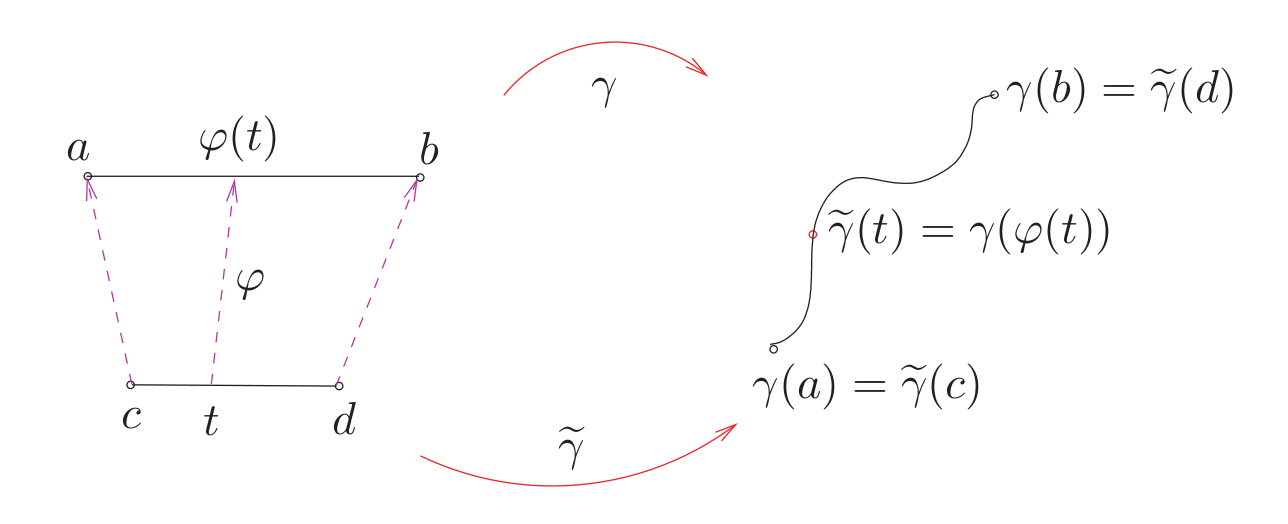
\includegraphics[scale=0.25]{equivalent_paths.png}
			\end{center}
			\begin{align*}
				\int_{\tilde{\gamma}}f\of{z}dz
				&=\int_a^bf\of{\tilde{\gamma}\of{t}}{\tilde{\gamma}'\of{t}}dt \\
				&=\int_a^bf\of{\gamma\of{\varphi\of{t}}}\gamma'\of{\varphi\of{t}}\varphi'\of{t}dt\\
				&=\int_c^df\of{\gamma\of{\tau}}\gamma'\of{\tau}d\tau\quad\text{by $\tau=\varphi\of{t}$}\\
				&=\int_{\gamma}f\of{z}dz.
			\end{align*}
		\end{proposition}
	\end{tcolorbox}
	
	\newpage
	\begin{tcolorbox}[colframe=thmcolor, title={\color{white}\bf An Important Integral}]
		\begin{theorem}
			Let $C$ be a circular path with center $z_0$ and radius $r>0$ traversed in the anti-clockwise direction. Then \[
			\int_C\of{z-z_0}^ndz=\begin{cases}
				2\pi i &:n= -1,\\
				0 &:n\neq -1.
			\end{cases}
			\]
		\end{theorem}
	\end{tcolorbox}
	\begin{proof}
		\begin{itemize}
			\item[(1)] Let $n\neq -1$ then
			\begin{align*}
				\int_C\of{z-z_0}^ndz&=\int_0^{2\pi}\of{z_0+re^{it}-z_0}^n\cdot ire^{it}dt\\
				&=\int_0^{2\pi}r^ne^{i nt}\cdot ire^{it}dt\\
				&=ir^{n+1}\int_0^{2\pi}e^{i(n+1)t}dt\\
				&=ir^{n+1}\left[\frac{1}{i(n+1)}e^{i(n+1)t}\right]_0^{2\pi}\\
				&=0.
			\end{align*}
			\item[(2)] Let $n = -1$ then
			\begin{align*}
				\int_C\of{z-z_0}^{-1}dz&=\int_0^{2\pi}\of{re^{it}}^{-1}\cdot ire^{it}dt\\
				&=\int_0^{2\pi}i dt\\
				&=2\pi i.
			\end{align*}
		\end{itemize}
	\end{proof}
	
	\begin{example}
		
	\end{example}
	
	\newpage
	\section{Properties of Contour Integration}
	
	\begin{tcolorbox}[colback=white,colframe=procolor,arc=5pt,title={\color{white}\bf Linearity of Integration}]
		\begin{proposition}
			Let $D$ be a domain in $\C$ and $\gamma:[a,b]\to D$ be a piecewise smooth path. Then the following hold: for all continuous $f,g:D\to\C$ and all $\alpha\in\C$, \[
			\int_\gamma\left(\alpha f+\beta g\right)\of{z}dz=\alpha\int_\gamma f\of{z}dz+\beta\int_\gamma g\of{z}dz.
			\]
		\end{proposition}
	\end{tcolorbox}
	\vspace{4pt}
	\begin{tcolorbox}[colback=white,colframe=procolor,arc=5pt,title={\color{white}\bf }]
		\begin{proposition}
			Let $\gamma:[a,b]\to D$ be a smooth path in a domain $D$ and $f:D\to\C$ be a continuous function. Then \[
			\int_{-\gamma}f\of{z}dz = -\int_{\gamma}f\of{z}dz.
			\]
		\end{proposition}
	\end{tcolorbox}
	\begin{proof}
		Note that $-\gamma:[a,b]\to\C$ is defined by \[
		\of{-\gamma}\of{t}=\gamma\of{a+b-t}.
		\]\begin{align*}
			\int_{-\gamma}f\of{z}dz &=\int_a^bf\of{\of{-\gamma}\of{t}}\of{-\gamma}'\of{t}dt\\
			&=\int_a^bf\of{\gamma\of{a+b-t}}\frac{d}{dt}\left[\of{-\gamma}\of{t}\right]dt\\
			&=\int_a^bf\of{\gamma\of{a+b-t}}\gamma'\of{a+b-t}\of{-1}dt\\
			&=\int_b^af\of{\gamma\of{\tau}}\gamma'\of{\tau}d\tau\quad\text{by $\tau:=a+b-t$, \ie, $d\tau=-dt$}\\
			&=-\int_a^bf\of{z}dz.
		\end{align*}
	\end{proof}
	\vspace{4pt}
	\begin{tcolorbox}[colback=white,colframe=procolor,arc=5pt,title={\color{white}\bf Concatenation of Paths}]
		\begin{proposition}
			Let $\gamma_1:[a_1,b_1]\to D$ and $\gamma_2:[a_2,b_2]\to D$ be two paths such that $\gamma_1\of{b_1}=\gamma_2\of{a_2}$. Define the concatenation of paths $\gamma_1+\gamma_2:\left[a_1,b_1+b_2-a_2\right]$ as follows: \[
			\of{\gamma_1+\gamma_2}\of{t}=\begin{cases}
				\gamma_1\of{t} &:t\in[a_1,b_1],\\
				\gamma_2\of{t-b_1+a_2} &:t\in[b_1,b_1+b_2-a_2].
			\end{cases}
			\] Then \[
			\int_{\gamma_1+\gamma_2}f\of{z}dz=\int_{\gamma_1}f\of{z}dz+\int_{\gamma_2}f\of{z}dz.
			\]
		\end{proposition}
	\end{tcolorbox}
	\vspace{8pt}
	\begin{tcolorbox}[colback=white,colframe=procolor,arc=5pt,title={\color{white}\bf }]
		\begin{proposition}
			Let \begin{enumerate}
				\item $D$ be a domain in $\C$;
				\item $\gamma:[a,b]\to D$ be a piecewise smooth path and
				\item $f:D\to\C$ be a continuous function.
			\end{enumerate} Then \[
			\abs{\int_\gamma f\of{z}dz}\leq\of{\max_{t\in[a,b]}\abs{f\of{\gamma\of{t}}}}\cdot\int_\gamma\abs{dz}
			\]
		\end{proposition}
	\end{tcolorbox}
	\begin{proof}
		Consider first a curve $\varphi:[a,b]\to\C$. We claim that \[
		\abs{\int_a^b\varphi\of{t}dt}\leq\int_a^b\abs{\varphi\of{t}}dt.
		\] Let $\displaystyle\int_a^b\varphi\of{t}dt=re^{i\theta}$, where $r\geq 0$ and $\theta\in(-\pi,\pi]$. Then \begin{align*}
			\abs{\int_a^b\varphi\of{t}dt}=r
			&=e^{-i\theta}\int_a^b\varphi\of{t}dt\quad\because\int_a^b\varphi\of{t}dt=re^{i\theta}\\
			&=\int_a^be^{-i\theta}\varphi\of{t}dt\\
			&=\int_a^b\Re\of{e^{-i\theta}\varphi\of{t}}dt\quad\because\abs{\int_a^b\varphi\of{t}dt}\in\R\\
			&\leq\int_a^b\abs{\Re\of{e^{-i\theta}\varphi\of{t}}}dt \\
			&\leq\int_a^b\abs{\of{e^{-i\theta}\varphi\of{t}}}dt\quad\because\abs{\Re\of{z}}\leq\abs{z}\\
			&=\int_a^b\abs{\varphi\of{t}}dt\quad\because \abs{e^{-i\theta}}=1.
		\end{align*}
		
		Let $\varphi\of{t}:=f\of{\gamma\of{t}}\cdot\gamma'\of{t}$ with $t\in[a,b]$. Then
		\begin{align*}
			\abs{\int_\gamma f\of{z}dz}&=\abs{\int_a^b f\of{\gamma\of{t}}\gamma'\of{t}dt}\\
			&\leq{\int_a^b \abs{f\of{\gamma\of{t}}\gamma'\of{t}}dt}\\
			&=\int_a^b\abs{f\of{\gamma\of{t}}}\abs{\gamma'\of{t}}dt\\
			&\leq\max_{t\in[a,b]}\abs{f\of{\gamma\of{t}}}\cdot\int_a^b\abs{\gamma'\of{t}}dt.
		\end{align*}
	\end{proof}
	
	\section{Fundamental Theorem of Contour Integration}
	
	\begin{tcolorbox}[colback=white,colframe=thmcolor,arc=5pt,title={\color{white}\bf Fundamental Theorem of Contour Integration}]
		\begin{theorem}
			Let \begin{enumerate}[(i)]
				\item $D$ be a domain in $\C$;
				\item $\gamma:[a,b]\to D$ be a piecewise smooth path;
				\item $f:D\to\C$ be a continuous in $D$;
				\item $F:D\to\C$ be a holomorphic function such that $F'=f$ in $D$.
			\end{enumerate} Then \[
			\int_\gamma f\of{z}dz=F\of{\gamma\of{b}}-F\of{\gamma\of{a}}.
			\]
		\end{theorem}
	\end{tcolorbox}
	\begin{proof}
		For $z=x+iy\in D$, where $x,y\in\R$, we define the real-valued functions $U,V,u,v$ by \begin{align*}
			F(x+iy)&=U(x,y)+iV(x,y),\\
			f(x+iy)&=u(x,y)+iv(x,y).
		\end{align*} Also, set $\gamma\of{t}=x\of{t}+iy\of{t}$ ($t\in[a,b]$). Then
		\begin{align*}
			\int_\gamma f\of{z}dz&=\int_a^bf\of{\gamma\of{t}}\gamma'\of{t}dt\\
			&=\int_a^b\of{u+iv}\of{x'+iy'}dt\\
			&=\int_a^b\of{ux'-vy'}dt +i\int_a^b\of{vx'+uy'}dt\\
			&=\int_a^b\of{U_xx'-V_xy'}dt +i\int_a^b\of{V_xx'+U_xy'}dt\quad\because F'=U_x+iV_x=f=u+iv\\
			&=\int_a^b\of{U_xx'+U_yy'}dt +i\int_a^b\of{V_xx'+V_yy'}dt\quad\text{by CR-Eqs: $U_x=V_y$ and $U_y=-V_x$}\\
			&=\int_a^b\frac{d}{dt}\left[U(x,y)\right]dt+i\int_a^b\frac{d}{dt}\left[V(x,y)\right]dt\\
			&=U\of{x(b),y(b)}-U\of{x(a),y(a)}+i\of{V\of{x(b),y(b)}-V\of{x(a),y(a)}}\\
			&=\of{U\of{x(b),y(b)}+U\of{x(a),y(a)}}-\of{V\of{x(b),y(b)}+V\of{x(a),y(a)}}\\
			&=F\of{\gamma\of{b}}-F\of{\gamma\of{a}}.
		\end{align*}
	\end{proof}
	
	
	\newpage
	\section{The Cauchy Integral Theorem}
	
	\begin{tcolorbox}[colback=white,colframe=defcolor,arc=5pt,title={\color{white}\bf Path Homotopy}]
		\begin{definition}
			Consider two closed paths $\gamma_0,\gamma_1:[0,1]\to D$. $\gamma_0$ is \textit{$D$-homotopic to} $\gamma_1$ if there exists a continuous function $H:[0,1]^2\to D$ such that \begin{enumerate}[(H1)]
				\item $\forall t\in[0,1]: H(t,0)=\gamma_0(t)$;
				\item $\forall t\in[0,1]: H(t,1)=\gamma_1(t)$;
				\item $\forall s\in[0,1]: H(0,s)=H(1,s)$.
			\end{enumerate}
		\end{definition}
	\end{tcolorbox}
	\vspace{8pt}
	\begin{example}
		
	\end{example}	
	\vspace{8pt}
	\begin{tcolorbox}[colback=white,colframe=thmcolor,arc=5pt,title={\color{white}\bf The Cauchy Integral Theorem}]
		\begin{theorem}
			Let \begin{enumerate}[(i)]
				\item $D$ be a domain in $\C$;
				\item $f:D\to\C$ be holomorphic in $D$, and
				\item $\gamma_0,\gamma_1:[0,1]\to\C$ be two closed, piecewise smooth, $D$-homotopic paths.
			\end{enumerate} Then \[
			\int_{\gamma_0}f\of{z}dz=\int_{\gamma_1}f\of{z}dz.
			\]
		\end{theorem}
	\end{tcolorbox}
	\begin{proof}
		Consider a path homotopy $H:[0,1]^2\to D$ s.t. $H\in C^2$. Let $\gamma_s:=H\of{\cdot, s}$ be a closed path with fixed point $s$. Define \[
		I\of{s}:=\int_{\gamma_s}f\of{z}dz,\quad s\in[0,1].
		\] We must show that $I(0)=I(1)$. Note that \[
		\left[\forall s\in[0,1]:\frac{d}{ds}\left[I(s)\right]=0\right]\implies I(0)=I(1).
		\] We claim that $\displaystyle\frac{d}{ds}\left[I(s)\right]=0$ for $s\in[0,1]$:
		\begin{align*}
			\frac{d}{ds}\left[I(s)\right]&=\frac{d}{ds}\left[\int_{\gamma_s}f\of{z}dz\right]\\
			&=\frac{d}{ds}\left[\int_0^1f\of{\gamma_s\of{t}}\gamma_s'\of{t}dt\right]\\
			&=\frac{d}{ds}\left[\int_0^1f\of{H\of{t,s}}H_t\of{t,s}dt\right]\\
			&=\int_0^1\frac{\partial}{\partial s}\left[f\of{H\of{t,s}}\frac{\partial}{\partial t}H\of{t,s}\right]dt\\
			&=\int_0^1\left(f'\of{H(t,s)}\cdot \frac{\partial}{\partial s}H\of{t,s}\cdot \frac{\partial}{\partial t}H\of{t,s}+f\of{H(t,s)}\cdot \frac{\partial^2}{\partial s\partial t}H\of{t,s}\right)dt\\
			&=\int_0^1\frac{\partial}{\partial t}\left[f\of{H(t,s)}\frac{\partial }{\partial s}H\of{t,s}\right]dt\quad\because H\in C^2\\
			&=\left[f\of{H(t,s)}\frac{\partial }{\partial s}H\of{t,s}\right]_0^1\\
			&=f\of{H\of{1,s}}\frac{\partial}{\partial s}H\of{1,s}-f\of{H\of{0,s}}\frac{\partial}{\partial s}H\of{0,s}\\
			&=0,
		\end{align*} since \begin{enumerate}[(i)]
			\item By (H3), $H\of{1,s}=H\of{0,s}$ holds.
			\item $\displaystyle\frac{\partial}{\partial s}H\of{1,s}=\lim_{h\to 0}\frac{H\of{1,s+h}-H\of{1,s}}{h}=\lim_{h\to 0}\frac{H\of{0,s+h}-H\of{0,s}}{h}=\frac{\partial}{\partial s}H\of{0,s}$.
		\end{enumerate}
		Hence \[
		\frac{d}{ds}\left[I\of{s}\right]=0\implies I\of{0}=I\of{1}\implies
		\int_{\gamma_0}f\of{z}dz=\int_{\gamma_1}f\of{z}dz.
		\]
	\end{proof}
	\vspace{8pt}
	\begin{tcolorbox}[colback=white,colframe=thmcolor,arc=5pt,title={\color{white}\bf Cauchy-Goursat Theorem}]
		\begin{theorem}
			Let $f:D\to\C$ be a holomorphic function, where $D\subseteq\C$ is a simply connected domain. Let $C$ be a closed contour in $D$. Then \[
			\oint_C f\of{z}dz = 0.
			\]
		\end{theorem}
	\end{tcolorbox}
	
	\begin{tikzpicture}[scale=1.5]
		
		% Connected and simply connected
		\filldraw[fill=green!20] (0,0) ellipse (1cm and 0.5cm);
		\draw (0.8,0) node {$D$};
		\draw (0,-1) node {Connected (\textcolor{blue}{O})};
		\draw (0,-1.4) node {Simply connected (\textcolor{blue}{O})};
		
		% Non-connected and simply connected
		\filldraw[fill=green!20] (4.5,0) circle (0.4cm);
		\draw (4.5,0) node {$D_1$};
		\filldraw[fill=green!20] (3.5,0) circle (0.4cm);
		\draw (3.5,0) node {$D_2$};
		\draw (4,-1) node {Connected (\textcolor{red}{X})};
		\draw (4,-1.4) node {Simply connected (\textcolor{blue}{O})};
		
		% Connected and non simply connected
		\filldraw[fill=green!20] (0,-3) ellipse (1cm and 0.7cm);
		\draw (0.8,-3) node {$D$};
		\draw (0,-4) node {Connected (\textcolor{blue}{O})};
		\draw (0,-4.4) node {Simply connected (\textcolor{red}{X})};
		\filldraw[fill=white] (0,-3) circle (0.2cm);
		
		% Non-connected and non simply connected
		\filldraw[fill=green!20] (4.8,-3) circle (0.6cm);
		\draw (4.8,-3) node {$D_1$};
		\filldraw[fill=green!20] (3.2,-3) circle (0.6cm);
		\filldraw[fill=white] (3.2,-3) circle (0.1cm);
		\draw (3.5,-3) node {$D_2$};
		\draw (4,-4) node {Connected (\textcolor{red}{X})};
		\draw (4,-4.4) node {Simply connected (\textcolor{red}{X})};
		
	\end{tikzpicture}
	
	\newpage
	\section{Existence of Primitive}
	
	
	\begin{tcolorbox}[colback=white,colframe=thmcolor,arc=5pt,title={\color{white}\bf Anti-derivative Theorem}]
		\begin{theorem}
			Let \begin{enumerate}[(i)]
				\item $D$ is a simply connected domain and
				\item $f:D\to\C$ is holomorphic.
			\end{enumerate} Then there is a holomorphic function $F:D\to\C$ such that \[
			z\in D\implies F'\of{z}=f\of{z}.
			\]
		\end{theorem}
	\end{tcolorbox}
	\begin{proof}
		Fixed a point $p\in D$. Define a function $F:D\to\C$ as follows: \[
		F\of{z}=\int_{\gamma_z}f\of{\zeta}d\zeta
		\] where $\gamma_z$ is a path joining $p$ to $z$. \begin{enumerate}[(i)]
			\item ($F$ is well-defined) Clearly, $\gamma:=\gamma_z+\of{-\tilde{\gamma_z}}$ is closed. Then
			\begin{align*}
				\int_{\gamma}f\of{\zeta}d\zeta=0&\implies \int_{\gamma_z+\of{-\tilde{\gamma_z}}}f\of{\zeta}d\zeta=0\\
				&\implies\int_{\gamma}f\of{\zeta}d\zeta=\int_{\tilde{\gamma_z}}f\of{\zeta}d\zeta
			\end{align*} That is, Cauchy Integral Theorem gives $F$ is well-defined.
			\item (Holomorphicity of $F$ and $F'=f$ in $D$) Since $f$ is holomorphic in $D$, it is also continuous there. Let $\varepsilon>0$. Then \[
			\exists\delta>0:\forall z\in D:\abs{w-z}<\delta\implies\abs{f\of{w}-f\of{z}}<\varepsilon.
			\] We take a $w$ such that $0<\abs{w-z}<\delta$. Then \[
			\frac{F\of{w}-F\of{z}}{w-z}=\frac{1}{w-z}\of{\int_{\gamma_w}f\of{\zeta}d\zeta-\int_{\gamma_z}f\of{\zeta}d\zeta}.
			\] Let $\gamma_{zw}$ is a straight line path joining $z$ to $w$. By the Cauchy Integral Theorem, we obtain \[
			0=\int_{\gamma_z+\gamma_{zw}-\gamma_w}f\of{\zeta}d\zeta\implies\int_{\gamma_{zw}}f\of{\zeta}d\zeta=\int_{\gamma_w}f\of{\zeta}d\zeta-\int_{\gamma_z}f\of{\zeta}d\zeta.
			\] Note that \[
			w-z=\zeta\bigg|_z^w=\int_{\gamma_{zw}}\frac{d}{d\zeta}\left[\zeta\right] d\zeta=\int_{\gamma_{zw}}1d\zeta.
			\]Then \begin{align*}
				\frac{F\of{w}-F\of{z}}{w-z}-f\of{z}&=\frac{1}{w-z}\int_{\gamma_{zw}}f\of{\zeta}d\zeta-f\of{z}\\
				&=\frac{1}{w-z}\int_{\gamma_{zw}}f\of{\zeta}d\zeta-f\of{z}\cdot\frac{1}{w-z}\int_{\gamma_{zw}}1d\zeta\\
				&=\frac{1}{w-z}\int_{\gamma_{zw}}\of{f\of{\zeta}-f\of{z}}d\zeta,
			\end{align*} and so \begin{align*}
				\abs{\frac{F\of{w}-F\of{z}}{w-z}-f\of{z}}&=\abs{\frac{1}{w-z}\int_{\gamma_{zw}}\of{f\of{\zeta}-f\of{z}}d\zeta}\\
				&=\frac{1}{\abs{w-z}}\abs{\int_{\gamma_{zw}}\of{f\of{\zeta}-f\of{z}}d\zeta}\\
				&\leq\frac{1}{\abs{w-z}}\cdot\max_{\zeta\in\gamma_{zw}}\abs{f\of{\zeta}-f\of{z}}\cdot\int_{\gamma_{zw}}\abs{dz}\\
				&<\frac{1}{\abs{w-z}}\cdot\varepsilon\cdot\abs{w-z}\\
				&=\varepsilon.
			\end{align*} Thus $F'\of{z}=f\of{z}$, and $F$ is holomorphic.
		\end{enumerate}
	\end{proof}
	
	\newpage
	\section{The Cauchy Integral Formula}
	
	\begin{tcolorbox}[colback=white,colframe=thmcolor,arc=5pt,title={\color{white}\bf The Cauchy Integral Formula for Circular Paths}]
		\begin{theorem}
			Let \begin{enumerate}[(1)]
				\item $D$ be a domain;
				\item $f:D\to\C$ be holomorphic in $D\setminus\set{0}$, and continuous on $D$;
				\item the disk $\Delta:=\set{z\in\C:\abs{z-z_0}\leq r}\subset D$ with $r>0$ and $z_0\in D$.
			\end{enumerate} Then \[
			f\of{z_0}=\frac{1}{2\pi i}\int_{C_r}\frac{f\of{z}}{z-z_0}dz,\quad \abs{z-z_0}<r,
			\] where $C_r$ is the circular path $C_r\of{t}=z_0+re^{it}$, $t\in[0,2\pi]$, with enter $z_0$ and radius $r>0$ traversed in the anti-clockwise direction.
		\end{theorem}
	\end{tcolorbox}
	\begin{proof}
		Let $\varepsilon>0$. We must show that \[
		\abs{\frac{1}{2\pi i}\int_{C_r}\frac{f\of{z}}{z-z_0}dz-f\of{z_0}}<\varepsilon.
		\] The continuity of $f$ on $D$ gives \[
		\exists\delta:\abs{z-z_0}<\varepsilon\implies\abs{f\of{z}-f\of{z_0}}<\varepsilon.
		\] Since $C_r$ is $D\setminus\set{z_0}$-homotopic to $C_\delta$, we have \[
		\int_{C_r}\frac{f\of{z}}{z-z_0}dz=\int_{C_\delta}\frac{f\of{z}}{z-z_0}dz
		\] Note that \[
		\int\frac{1}{z-z_0}dz=2\pi i.
		\] Thus, \begin{align*}
			\abs{\frac{1}{2\pi i}\int_{C_r}\frac{f\of{z}}{z-z_0}dz-f\of{z_0}}&=
			\abs{\frac{1}{2\pi i}\int_{C_\delta}\frac{f\of{z}}{z-z_0}dz-f\of{z_0}}\\
			&=\abs{\frac{1}{2\pi i}\int_{C_\delta}\frac{f\of{z}}{z-z_0}dz-\frac{1}{2\pi i}\cdot f\of{z_0}\cdot\int_{C_\delta}\frac{1}{z-z_0}dz}\\
			&=\abs{\frac{1}{2\pi i}\int_{C_\delta}\frac{f\of{z}-f\of{z_0}}{z-z_0}dz}\\
			&\leq\frac{1}{\abs{2\pi i}}\cdot\max_{\substack{z\in C_\delta\\ (\abs{z-z_0}=\delta)}}\abs{\frac{f\of{z}-f\of{z_0}}{z-z_0}}\cdot\int_{C_\delta}\abs{dz}\\
			&<\frac{1}{2\pi}\cdot\frac{\varepsilon}{\delta}\cdot 2\pi\delta\\
			&=\varepsilon.
		\end{align*}
	\end{proof}
	
	
	\newpage
	\section{Holomorphic Functions are Infinitely Differentiable}
	
	\newpage
	\section{Liouville's Theorem; Fundamental Theorem of Algebra}
	
	\newpage
	\section{Morera's Theorem: converse to Cauchy's Integral Theorem}
	\begin{tcolorbox}[colback=white,colframe=defcolor,arc=5pt,title={\color{white}\bf Length of Curve}]
		
	\end{tcolorbox}\begin{tcolorbox}[colback=white,colframe=defcolor,arc=5pt,title={\color{white}\bf Length of Curve}]
		
	\end{tcolorbox}\begin{tcolorbox}[colback=white,colframe=defcolor,arc=5pt,title={\color{white}\bf Length of Curve}]
		
	\end{tcolorbox}\begin{tcolorbox}[colback=white,colframe=defcolor,arc=5pt,title={\color{white}\bf Length of Curve}]
		
	\end{tcolorbox}\begin{tcolorbox}[colback=white,colframe=defcolor,arc=5pt,title={\color{white}\bf Length of Curve}]
		
	\end{tcolorbox}\begin{tcolorbox}[colback=white,colframe=defcolor,arc=5pt,title={\color{white}\bf Length of Curve}]
		
	\end{tcolorbox}\begin{tcolorbox}[colback=white,colframe=defcolor,arc=5pt,title={\color{white}\bf Length of Curve}]
		
	\end{tcolorbox}\begin{tcolorbox}[colback=white,colframe=defcolor,arc=5pt,title={\color{white}\bf Length of Curve}]
		
	\end{tcolorbox}
	\begin{tcolorbox}[colback=white,colframe=defcolor,arc=5pt,title={\color{white}\bf Length of Curve}]
		\begin{definition}
			
		\end{definition}
	\end{tcolorbox}	

	\newpage
	\chapter{Taylor and Laurent series}
		
	\bibliographystyle{plain}
	\bibliography{references}	
	
	% End document
\end{document}
